% Provenance (never printed): see sources/outline_sources.md (Year 2: sedimentary basins;
% subsidence curves and backstripping; the stretching model). Stretching model after McKenzie
% (1978) as restated by Sheplev and Reverdatto (1998) and coded in pyBacktrack (EarthByte);
% backstripping after pyBacktrack's well module; North Sea after Sclater and Christie (1980);
% Michigan after Sloss (1982) and Crowe et al. (2009); the US Atlantic margin after Schlee et
% al. (1976), Poag (1979) and Lang et al. (2024); the Molasse after the chapter 13 rows.
% Curves and the invented well from figdata/bachelor-2/basins.py; exercise and problem values
% in the Book 4 scratch calculator calc/ch16.py.
\chapter{مقارنة بين الأحواض الرسوبية}\label{ch:b2:basins-compared}

قبالة ساحل شرق الولايات المتحدة، تحت الرصيف القاري، يحوي منخفض بالتيمور
كانيون ما لا يقل عن \qty{14}{km} من الصخر الرسوبي. والبئر المحفورة في ركام كهذا
تقرأ تاريخه بالعكس: فكل وحدة تعبرها كانت يومًا قاع البحر، على عمق تسجّله
الأحافير والرواسب، ثم دُفنت وانضغطت منذ ذلك الحين. وعمق كل سطح
مؤرَّخ نقطة على منحنى للهبوط. ومع ذلك فإن معظم الهبوط سبّبه
وزن الرواسب نفسها. ولمعرفة ما صنع الحوض، يجب أن يُرفع ذلك الوزن،
طبقة بعد طبقة. يبيّن هذا الفصل كيف، وما تقوله النتيجة عن الغلاف الصخري.
% ledger: poag79:bct, schlee76:atlantic

\begin{recall}
\textbf{من مجلد السنة الأولى}: الحوض الرسوبي، والهبوط والهبوط التكتوني،
والاستيعاب، والسكونية؛ والانضغاط، وفكّ الانضغاط وقانون أثي، والسمك الصلب
لطبقة؛ وحمل الرواسب، الذي يضخّم الهبوط بالعامل $(\rho_m - \rho_w)/(\rho_m - \rho_s)$؛
وتوازن إيري؛ والغلاف الصخري وتدرّجه الحراري؛ والشقوق القارية والهوامش السلبية.
\textbf{من مجلدات الفيزياء}: معادلة الحرارة وحلولها بمتسلسلات فورييه.
\textbf{من \cref{ch:b2:alpine-orogen}}: \omterm{def:b2:alpine-orogen:foreland}{الحوض الأمامي الجبلي}، \omterm{def:b2:alpine-orogen:foreland}{والفليش} \omterm{def:b2:alpine-orogen:foreland}{والمولاس}.
\end{recall}

\begin{omfigure}
\centering
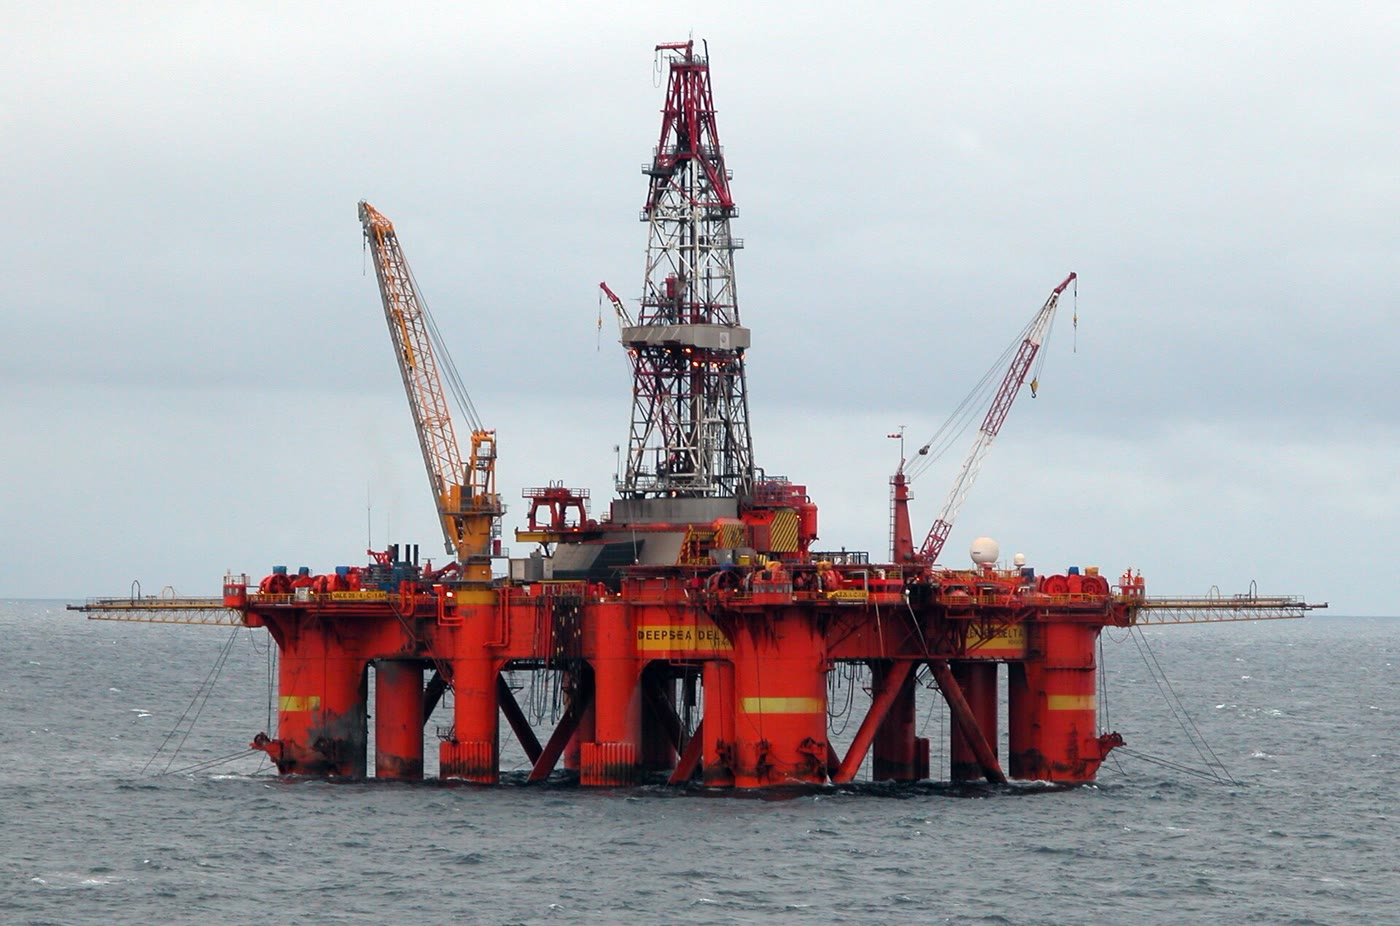
\includegraphics[width=0.66\linewidth]{images/book4/b2-16-drilling-rig.jpg}
\par\smallskip{\small منصّة حفر شبه غاطسة في بحر الشمال. والآبار المحفورة
من منصّات كهذه تعطي السماكات والأعمار وأنواع الصخور التي يُعاد منها بناء هبوط حوض.
الصورة: \mbox{\textdir TLT Erik Christensen, 2005, CC BY-SA 3.0}.}
\end{omfigure}

\section{الأحواض وما يجعلها تهبط}\label{sec:b2:basins-compared:types}

ميّز مجلد السنة الأولى الأحواض بحسب موقعها. أمّا هنا فتُميَّز بحسب ما يحرّك
هبوطها.

\begin{definition}[الأحواض داخل الكراتونية، وأحواض الشقّ، وأحواض الهامش السلبي]\label{def:b2:basins-compared:types}
\emph{الحوض داخل الكراتوني}\index{الحوض داخل الكراتوني} حوض واسع، دائري أو بيضوي، في
داخل قارة، بعيد عن حدود الصفائح، يهبط ببطء على مدى أزمنة طويلة جدًا
دون تصدّع كبير. و\emph{حوض الشقّ}\index{حوض الشقّ} حوض تحدّه صدوع عادية
في غلاف صخري قاري يُمطّ؛ ويتبع هبوطه التمطّط ثم
تبرّد الغلاف الصخري. و\emph{حوض الهامش السلبي}\index{حوض الهامش السلبي} هو
إسفين الرواسب، المتثخّن نحو المحيط، الذي يتراكم على هامش قاري بعد
الانفصال، فوق القشرة المرقّقة للشقّ القديم.
\end{definition}

يُكمل \omterm{def:b2:alpine-orogen:foreland}{الحوض الأمامي الجبلي} في \cref{ch:b2:alpine-orogen} القائمة، وتُترك الأحواض التي تنفتح
على امتداد الصدوع المضربية لمجلد السنة الثالثة. وثلاث آليات تجعل قاع
الحوض يهبط:
\begin{itemize}
  \item الترقيق \emph{الميكانيكي}: حين تُمطّ القشرة وتُرقّق بالصدوع، تحلّ محلّ
        القشرة الخفيفة مادة الوشاح الأكثف وينخفض السطح لاستعادة التوازن الأيزوستاتي؛
  \item الانكماش \emph{الحراري}: الغلاف الصخري الذي سُخّن، بالتمطّط أو من
        الأسفل، يبرد بعد ذلك، فيزداد كثافة ويهبط، ببطء، على مدى عشرات ملايين السنين؛
  \item \emph{التحميل}: وزن حزام دفعي، أو وزن الرواسب نفسها، يثني
        الغلاف الصخري نحو الأسفل؛ وذلك الانثناء ينتمي إلى مجلد السنة الثالثة، والصورة المحلية لحمل
        الرواسب، صورة إيري، تكفي هنا.
\end{itemize}
تجمع أحواض الشقّ بين الآليتين الأوليين، وترث الهوامش السلبية الثانية من مرحلة شقّها،
وتصنع الثالثةُ الأحواض الأمامية الجبلية. أمّا الأحواض داخل الكراتونية فهي الأقل فهمًا.

\begin{omfigure}
\centering
\begin{tikzpicture}[x=1cm, y=1cm, font=\scriptsize, line join=round,
  sed/.style={fill=yellow!35, draw=black!60, line width=0.3pt},
  crust/.style={fill=orange!25, draw=black!60, line width=0.3pt},
  mlith/.style={fill=green!12, draw=black!60, line width=0.3pt},
  asth/.style={fill=red!12, draw=black!60, line width=0.3pt},
  sea/.style={fill=blue!8, draw=none},
  ttl/.style={anchor=south west, font=\scriptsize\bfseries}]
% (a) intracratonic
\begin{scope}
\fill[asth] (0,-2.4) rectangle (6.6,-1.6);
\fill[mlith] (0,-1.6) rectangle (6.6,-0.7);
\fill[crust] (0,-0.7) -- (6.6,-0.7) -- (6.6,0) -- (4.9,0) .. controls (4.1,-0.45) and (2.5,-0.45) .. (1.7,0) -- (0,0) -- cycle;
\fill[sed] (1.7,0) .. controls (2.5,-0.45) and (4.1,-0.45) .. (4.9,0) -- cycle;
\draw[black!70] (0,0) -- (6.6,0);
\node[ttl] at (0,0.05) {\foreignlanguage{arabic}{(أ) داخل كراتوني}};
\node at (3.3,-1.15) {الغلاف الصخري الوشاحي};
\node at (3.3,-2.0) {الأستينوسفير};
\end{scope}
% (b) rift
\begin{scope}[xshift=7.2cm]
\fill[asth] (0,-2.4) -- (6.6,-2.4) -- (6.6,-1.6) -- (4.5,-1.6) -- (3.3,-1.0) -- (2.1,-1.6) -- (0,-1.6) -- cycle;
\fill[mlith] (0,-1.6) -- (2.1,-1.6) -- (3.3,-1.0) -- (4.5,-1.6) -- (6.6,-1.6) -- (6.6,-0.7) -- (4.4,-0.7) -- (3.3,-0.45) -- (2.2,-0.7) -- (0,-0.7) -- cycle;
\fill[crust] (0,-0.7) -- (2.2,-0.7) -- (3.3,-0.45) -- (4.4,-0.7) -- (6.6,-0.7) -- (6.6,0) -- (4.6,0) -- (4.25,-0.42) -- (3.75,-0.2) -- (3.35,-0.4) -- (2.95,-0.15) -- (2.45,-0.42) -- (2.0,0) -- (0,0) -- cycle;
\fill[sed] (2.0,0) -- (2.45,-0.42) -- (2.95,-0.15) -- (3.35,-0.4) -- (3.75,-0.2) -- (4.25,-0.42) -- (4.6,0) -- cycle;
\draw[thick] (2.0,0) -- (2.5,-0.5) (4.6,0) -- (4.2,-0.5) (2.95,-0.15) -- (3.4,-0.48);
\draw[black!70] (0,0) -- (6.6,0);
\node[ttl] at (0,0.05) {\foreignlanguage{arabic}{(ب) شقّ}};
\node at (1.45,-1.15) {الغلاف الصخري الوشاحي};
\node at (5.4,-2.0) {الأستينوسفير};
\end{scope}
% (c) passive margin
\begin{scope}[yshift=-3.3cm]
\fill[asth] (0,-2.4) -- (6.6,-2.4) -- (6.6,-1.2) -- (0,-1.6) -- cycle;
\fill[mlith] (0,-1.6) -- (6.6,-1.2) -- (6.6,-1.0) -- (4.2,-1.05) -- (2.4,-0.75) -- (0,-0.7) -- cycle;
\fill[crust] (0,-0.7) -- (2.4,-0.75) -- (4.2,-1.05) -- (4.2,-0.85) -- (2.6,-0.25) -- (1.6,0) -- (0,0) -- cycle;
\fill[gray!35, draw=black!60, line width=0.3pt] (4.2,-1.05) -- (6.6,-1.0) -- (6.6,-0.85) -- (4.2,-0.85) -- cycle;
\fill[sed] (1.6,0) -- (2.6,-0.25) -- (4.2,-0.85) -- (6.6,-0.85) -- (6.6,-0.55) -- (3.6,-0.45) -- (2.6,-0.05) -- (2.2,0) -- cycle;
\fill[sea] (2.2,0) -- (6.6,0) -- (6.6,-0.55) -- (3.6,-0.45) -- (2.6,-0.05) -- cycle;
\draw[black!70] (0,0) -- (2.2,0);
\draw[blue!60!black] (2.2,0) -- (6.6,0);
\node[ttl] at (0,0.05) {\foreignlanguage{arabic}{(ج) هامش سلبي}};
\node at (5.4,-0.95) {\tiny قشرة محيطية};
\node at (1.3,-2.0) {الأستينوسفير};
\node at (1.3,-1.05) {الغلاف الصخري الوشاحي};
\end{scope}
% (d) foreland
\begin{scope}[xshift=7.2cm, yshift=-3.3cm]
\fill[asth] (0,-2.4) -- (6.6,-2.4) -- (6.6,-2.0) -- (0,-1.5) -- cycle;
\fill[mlith] (0,-1.5) -- (6.6,-2.0) -- (6.6,-1.2) -- (0,-0.7) -- cycle;
\fill[crust] (0,-0.7) -- (6.6,-1.2) -- (6.6,-0.55) -- (3.6,-0.4) .. controls (2.0,-0.15) .. (0,0) -- cycle;
\fill[sed] (0,0) .. controls (2.0,-0.15) .. (3.6,-0.4) -- (6.6,-0.55) -- (5.0,0) -- cycle;
\fill[crust, fill=orange!45] (5.0,0) -- (6.6,-0.55) -- (6.6,0.6) -- (6.1,0.6) -- cycle;
\draw[thrust fault] (6.6,-0.55) -- (5.0,0);
\draw[black!70] (0,0) -- (5.0,0);
\node[ttl] at (0,0.05) {\foreignlanguage{arabic}{(د) أمامي جبلي}};
\node[anchor=north east, font=\tiny] at (6.55,0.55) {الحزام};
\node at (2.2,-1.25) {الغلاف الصخري الوشاحي};
\node at (1.5,-2.05) {الأستينوسفير};
\end{scope}
\end{tikzpicture}
\par\smallskip{\small أربع عائلات من الأحواض في مقاطع تخطيطية عبر الغلاف الصخري (دون
مقياس رسم؛ الرواسب بالأصفر، والقشرة القارية بالبرتقالي، والقشرة المحيطية بالرمادي). والمبالغة
الرأسية كبيرة: فالأحواض الحقيقية عرضها مئات الكيلومترات وعمقها من بضعة إلى خمسة عشر
كيلومترًا.}
\end{omfigure}

أحواض الشقّ في بحر الشمال هي الحالة الكلاسيكية للآليتين الأوليين. فقد تكوّنت فيه
غرابن منذ الترياسي، ودام آخر تمطّط كبير من الجوراسي الأوسط
إلى منتصف الطباشيري؛ ثم هدأت الصدوع، واستمر وسط الحوض في الهبوط
كصحن واسع، ملأته الطباشير والأحجار الرملية، وفي معظم الحقب الثالث، الطين الصفحي
والحجر الطيني. ولو حُمّلت قاعدته بالماء وحده، لهبطت 1100 إلى
\qty{1400}{m} أخرى في الوسط و600 إلى \qty{700}{m} على الجانبين بعد توقّف التصدّع.
% ledger: sc80b4:north-sea

ويُظهر الهامش السلبي لشرق الولايات المتحدة الهبوط نفسه على نطاق أكبر.
فالمقاطع الزلزالية عبر الرصيف تُظهر أكثر من \qty{14}{km} من صخور الميزوزوي والأحدث منها في
منخفض بالتيمور كانيون و\qty{8}{km} في حوض جورجز بانك، في وحدات تتثخّن
نحو المحيط. وتتبع مراكز ترسّبه الجوراسية بنى الشقّ ونطاقات
هبوطه الحراري اللاحق.
% ledger: schlee76:atlantic, lang24:atlantic

حوض ميشيغان هو النموذج المرجعي للأحواض داخل الكراتونية. بيضوي، مساحته بضع مئات الآلاف
من الكيلومترات المربعة، ويحوي أكثر من \qty{4}{km} من رواسب الدهر الظاهر ترسّبت
في نوبات متمايزة على مدى نحو 500 مليون سنة، مع قليل من التصدّع. ونوبات هبوطه
الأسرع تتزامن مع نوبات أحواض أخرى في دواخل أمريكا الشمالية وقارات
أخرى، ما يوحي بسبب أكبر من حوض واحد. \omterm{def:b2:basins-compared:backstripping}{والتجريد العكسي} لأكثر من 57\,000
سجلّ آبار يُظهر نمط هبوط طويل العمر شبه دائري، يقترح المؤلّفون أن
هبوطًا وشاحيًا نحو الأسفل قد يفسّره، تقطعه أزمنة تكوّنين جبليين على الهامش
البعيد للقارة. ولا يزال سبب هبوط الأحواض داخل الكراتونية موضع خلاف.
% ledger: sloss82:michigan, crowe09:michigan

\section{منحنيات الهبوط}\label{sec:b2:basins-compared:curves}

تعطي البئر، أو المقطع المقيس، لكل وحدة عمقها الحالي ونوع صخرها وعمرها،
مقروءًا من الأحافير أو من المضاهاة. ومع عمق الماء الذي ترسّبت فيه كل وحدة،
مقروءًا من أحافيرها وبناها الرسوبية، تعطي تاريخ الحوض.

\begin{definition}[منحنى الهبوط]\label{def:b2:basins-compared:curve}
\emph{منحنى الهبوط}\index{منحنى الهبوط} لحوض في موقع ما هو التمثيل البياني لعمق
سطح مرجعي، هو عادة القاعدة أو قاعدة أقدم وحدة، تحت مستوى سطح البحر،
بدلالة الزمن. ويستعمل منحنى الهبوط \emph{الكلي} سمك الرواسب كما كان في كل
زمن، مضافًا إليه عمق الماء؛ أمّا منحنى الهبوط \emph{التكتوني} فيستبدل بالرواسب ماءً
ويزيل أثرها الأيزوستاتي.
\end{definition}

لم تكن الوحدة في الماضي بسمكها اليوم قطّ. فبعد دفنها فقدت مساميتها؛ ولم تتغيّر حبيباتها،
لكن ماءها عُصر. وقد كتب مجلد السنة الأولى المسامية على العمق
$z$ بقانون أثي، $\phi(z) = \phi_0\,e^{-z/c}$، ووجد السمك الصلب لطبقة بين
$z_1$ و$z_2$،
\[
  T_s = (z_2 - z_1) - \phi_0 c\left(e^{-z_1/c} - e^{-z_2/c}\right),
\]
الذي يبقى ثابتًا حين تتحرّك الطبقة. و\emph{لفكّ انضغاط} وحدة إلى موضع أقل عمقًا،
مع قمّتها الآن عند $z_1'$، يُبحث عن القاعدة $z_2'$ التي تحفظ السمك الصلب نفسه. وليس
للمعادلة حلّ مغلق، لكن التكرار بالنقطة الثابتة
\[
  z_2' \leftarrow z_1' + T_s + \phi_0 c\left(e^{-z_1'/c} - e^{-z_2'/c}\right)
\]
ابتداءً من $z_2' = z_1' + T_s$ يتقارب في بضع خطوات. وكتلة الطبقة لكل وحدة مساحة
هي كتلة حبيباتها مضافًا إليها كتلة ماء مسامّها،
\[
  m = \rho_g T_s + \rho_w\,(z_2 - z_1 - T_s),
\]
حيث $\rho_g$ كثافة الحبيبات؛ وقسمة كتلة عمود على سمكه تعطي
كثافته المتوسطة $\bar\rho_s$.

للصخارات المستعملة في هذا الفصل، الرمل والطين الصفحي والطباشير والرمل الطيني، يعطي الجدول أدناه
ثوابت سكلاتر وكريستي (1980)، كما هي مضمّنة في برنامج مفتوح المصدر.
يحتفظ الرمل بمساميته إلى أعمق مدى، ويفقدها الطباشير أسرع.
% ledger: pybacktrack:compaction

\begin{center}
\small
\begin{tabular}{lccc}
\hline
الصخارة & كثافة الحبيبات (\unit{kg.m^{-3}}) & المسامية السطحية $\phi_0$ & طول التناقص $c$ (\unit{m}) \\
\hline
رمل & 2650 & 0.49 & 3704 \\
طين صفحي & 2700 & 0.63 & 1960 \\
طباشير & 2710 & 0.70 & 1408 \\
رمل طيني & 2680 & 0.56 & 2564 \\
\hline
\end{tabular}
\end{center}

\section{التجريد العكسي}\label{sec:b2:basins-compared:backstripping}

يمزج \omterm{def:b2:basins-compared:curve}{منحنى الهبوط} الكلي سببين: ما صنع الحوض أيًّا كان، ووزن ما
ملأه. والفصل بينهما هو غرض الإجراء التالي، الأداة المركزية لتحليل
الأحواض.

\begin{definition}[التجريد العكسي]\label{def:b2:basins-compared:backstripping}
\emph{التجريد العكسي}\index{التجريد العكسي} هو إعادة بناء الهبوط التكتوني لحوض
عبر الزمن: تُزال وحدات البئر واحدة تلو الأخرى، بدءًا بالأحدث،
ويُفكّ انضغاط الباقية في كل خطوة، ويُزال الأثر الأيزوستاتي لحمل الرواسب والماء
للحصول على العمق الذي كانت القاعدة ستقف عنده تحت الماء وحده.
\end{definition}

الخطوة الأخيرة توازن أيزوستاتي. وقد أجراه مجلد السنة الأولى لحوض ممتلئ حتى مستوى سطح البحر؛
والحالة العامة تضيف عمق الماء ومستوى البحر.

\begin{proposition}[التجريد العكسي وفق إيري]\label{prop:b2:basins-compared:backstrip}
ليحوِ حوض، في زمن ما، عمودًا رسوبيًا سمكه $S$ وكثافته المتوسطة
$\bar\rho_s$، تحت عمق ماء $W_d$، بينما كان البحر أعلى من مستواه الحالي بمقدار $\Delta_{SL}$.
في توازن أيزوستاتي محلي فوق وشاح كثافته $\rho_m$، ومع ماء كثافته $\rho_w$، يكون
الهبوط التكتوني في ذلك الزمن، مقيسًا من مستوى سطح البحر الحالي، هو
\[
  Y = S\,\frac{\rho_m - \bar\rho_s}{\rho_m - \rho_w} + W_d
      - \Delta_{SL}\,\frac{\rho_m}{\rho_m - \rho_w}.
\]
\end{proposition}

\begin{proof}
قارن عمودين فوق الغلاف الصخري نفسه، حتى عمق تعويض تحتهما كليهما. في
الأول، ماء عمقه $W_d$ فوق رواسب سمكها $S$؛ وفي الثاني، يملأ الماء
وحده حوضًا عمقه $Y'$ تحت سطح البحر نفسه. وكتلتاهما متساويتان:
\[
  \rho_w W_d + \bar\rho_s S + \rho_m\,(d - W_d - S) = \rho_w Y' + \rho_m\,(d - Y'),
\]
حيث $d$ العمق المشترك لمستوى التعويض تحت سطح البحر. ومنه
$Y'(\rho_m - \rho_w) = S(\rho_m - \bar\rho_s) + W_d(\rho_m - \rho_w)$، وهما الحدّان
الأولان. وإذا كان البحر أعلى من اليوم بمقدار $\Delta_{SL}$، فذلك الماء الإضافي ليس جزءًا من
هبوط الحوض الذاتي: فبإزالته ترتفع القاعدة المحمّلة بالماء بمقدار
$\Delta_{SL}\rho_w/(\rho_m - \rho_w)$، ويصغر عمقها تحت مستوى سطح البحر الحالي مرة أخرى بمقدار
$\Delta_{SL}$؛ والمجموع $\Delta_{SL}\,\rho_m/(\rho_m - \rho_w)$.
\end{proof}
% ledger: pybacktrack:backstrip

مع $\rho_m = \qty{3330}{kg.m^{-3}}$ و$\rho_w = \qty{1030}{kg.m^{-3}}$، يُحسب عمود من رواسب
كثافتها المتوسطة \qty{2300}{kg.m^{-3}} بالجزء $1030/2300 = 0.45$ من سمكه في الهبوط
التكتوني: فأكثر من نصف سمك ملء الحوض يفسح له المجال وزنه الذاتي.
والبحر الأعلى من اليوم بمقدار \qty{100}{m} يُنقص النتيجة بمقدار \qty{145}{m}. وعمق الماء
ومستوى البحر في الماضي هما أضعف المعطيات: فالأحافير تعطي مدى لأعماق الماء، يبلغ عرضه
غالبًا مئات الأمتار على المنحدر، ويرث الهبوط التكتوني ذلك المدى.

\begin{method}[التجريد العكسي لبئر]\label{met:b2:basins-compared:backstrip}
\begin{enumerate}
  \item عدّد الوحدات من القاعدة، مع الأعماق الحالية لقممها وقواعدها، وثوابت
        صخارتها $(\rho_g, \phi_0, c)$، وأعمار قممها، وعمق الماء عند
        كل عمر من تلك الأعمار.
  \item احسب السمك الصلب $T_s$ لكل وحدة من أعماقها الحالية.
  \item لعمر قمّة الوحدة $k$، أزل كل الوحدات الأحدث. ضع قمّة الوحدة
        $k$ عند العمق صفر وفكّ انضغاطها؛ ثم ضع كل وحدة أقدم، بالدور، تحت التي فوقها
        وفكّ انضغاطها.
  \item اجمع السماكات للحصول على $S$، والكتل للحصول على الكثافة المتوسطة
        $\bar\rho_s = \sum m / S$.
  \item طبّق \cref{prop:b2:basins-compared:backstrip} للحصول على $Y$؛ والهبوط الكلي هو
        $S + W_d$.
  \item كرّر لكل عمر، من الأقدم إلى الحاضر؛ وارسم $Y$ و$S + W_d$ بدلالة العمر.
\end{enumerate}
\end{method}

يبيّن الشكل أدناه النتيجة لبئر مختلقة في حوض شقّ. فقد أُخذت لُباب أربع وحدات:
رمل متزامن مع التصدّع ترسّب بينما كانت الصدوع نشطة، بين 165 و\qty{150}{Ma}؛ ثم طين صفحي،
وطباشير، ورمل طيني. واليوم لا حاجة إلى فكّ الانضغاط: فالقاعدة تقع على عمق \qty{6030}{m}
وللعمود كثافة متوسطة قدرها \qty{2358}{kg.m^{-3}}، فيكون $Y = \qty{2648}{m}$ تحت
\qty{100}{m} من الماء. وعند \qty{150}{Ma}، كان سمك الرمل وحده، بعد فكّ انضغاطه عند السطح،
\qty{2239}{m}، بكثافة متوسطة قدرها \qty{2055}{kg.m^{-3}}: وتحت \qty{200}{m} من الماء،
$Y = \qty{1441}{m}$. والهبوط الكلي
أكثر من ضعف الهبوط التكتوني، ويُظهر المنحنى التكتوني مرحلة أولى سريعة، ثم
هبوطًا متباطئًا: وهو شكل الشقّ.
% values (script): figdata/bachelor-2/basins.py part numbers (S_150 2239.5, rho_0 2357.9, Y_0 2648.7, Y_150 1442.1); printed from the rounded chain of calc/ch16.py (rho 2358 -> 2648; T 2239, rho 2055 -> 1441), as in the problem

\begin{omfigure}
\centering
% figdata/bachelor-2/basins.py parts stages and fit (invented well)
\begin{tikzpicture}
\begin{axis}[width=0.8\linewidth, height=6.0cm, x dir=reverse, y dir=reverse, xmin=0, xmax=170,
  ymin=0, ymax=6500, xlabel={العمر \babelsublr{(\unit{Ma})}}, ylabel={العمق تحت مستوى سطح البحر \babelsublr{(\unit{m})}},
  tick label style={font=\scriptsize}, label style={font=\small}, xtick={0,25,...,175},
  xtick pos=bottom, ytick pos=left,
  legend style={at={(0.5,1.04)}, anchor=south, draw=none, font=\scriptsize, legend columns=3,
  /tikz/every even column/.append style={column sep=8pt}}]
\addplot[omThm, line width=1pt, mark=*, mark size=1.6pt] table[x=age_Ma, y=total_m]
  {figdata/out/bachelor-2-basins-stages.dat};
\addlegendentry{\foreignlanguage{arabic}{الهبوط الكلي $S + W_d$}}
\addplot[blue!70!black, line width=1pt, mark=square*, mark size=1.6pt] table[x=age_Ma, y=Y_m]
  {figdata/out/bachelor-2-basins-stages.dat};
\addlegendentry{\foreignlanguage{arabic}{الهبوط التكتوني $Y$}}
\addplot[black!70, dashed, line width=0.8pt] table[x=age_Ma, y=Y_m]
  {figdata/out/bachelor-2-basins-fit.dat};
\addlegendentry{\foreignlanguage{arabic}{نموذج التمطّط، $\beta = 1.50$}}
\node[font=\scriptsize, anchor=south west] at (axis cs:149,1500) {نهاية التصدّع};
\end{axis}
\end{tikzpicture}
\par\smallskip{\small \omterm{def:b2:basins-compared:backstripping}{التجريد العكسي} لبئر مختلقة ذات أربع وحدات (المعطيات في مسألة نهاية
الأسبوع): عمق القاعدة مع الرواسب كما كانت في كل زمن، والهبوط التكتوني،
مع منحنى \omterm{def:b2:basins-compared:stretching}{نموذج التمطّط} الموفَّق على الهبوط عند نهاية التصدّع
(\cref{sec:b2:basins-compared:stretching}).}
\end{omfigure}

\begin{omfigure}
\centering
\begin{tikzpicture}[x=1cm, y=0.1cm, font=\scriptsize, line join=round,
  u/.style={draw=black!60, line width=0.3pt}]
% today
\begin{scope}
\fill[blue!8] (0,0) rectangle (1.6,-1.0);
\fill[u, fill=yellow!25] (0,-1.0) rectangle (1.6,-18.0);
\fill[u, fill=green!18] (0,-18.0) rectangle (1.6,-34.1);
\fill[u, fill=gray!25] (0,-34.1) rectangle (1.6,-45.2);
\fill[u, fill=yellow!55] (0,-45.2) rectangle (1.6,-61.3);
\draw[black!70] (0,-61.3) -- (1.6,-61.3);
\node[anchor=south] at (0.8,0.1) {اليوم};
\node at (0.8,-9.5) {رمل طيني};
\node at (0.8,-26) {طباشير};
\node at (0.8,-39.6) {طين صفحي};
\node at (0.8,-53.2) {رمل};
\node[anchor=north] at (0.8,-61.5) {\qty{6130}{m}};
\end{scope}
% at 150 Ma
\begin{scope}[xshift=3.0cm]
\fill[blue!8] (0,0) rectangle (1.6,-2.0);
\fill[u, fill=yellow!55] (0,-2.0) rectangle (1.6,-24.39);
\draw[black!70] (0,-24.4) -- (1.6,-24.4);
\node[anchor=south] at (0.8,0.1) {\qty{150}{Ma}};
\node at (0.8,-13.2) {رمل};
\node[anchor=north] at (0.8,-24.6) {\qty{2439}{m}};
\end{scope}
\draw[-{Latex}, thick] (4.9,-12) -- (6.1,-12) node[midway, above] {إزالة الحمل};
% water loaded
\begin{scope}[xshift=6.3cm]
\fill[blue!20] (0,0) rectangle (1.6,-14.4);
\draw[black!70] (0,-14.4) -- (1.6,-14.4);
\node[anchor=south] at (0.8,0.1) {ماء فقط};
\node at (0.8,-7.2) {ماء};
\node[anchor=north] at (0.8,-14.6) {$Y = \qty{1441}{m}$};
\end{scope}
\draw[black!40, dashed] (-0.3,0) -- (8.2,0);
\node[anchor=west] at (8.2,0) {مستوى سطح البحر};
\end{tikzpicture}
\par\smallskip{\small \omterm{def:b2:basins-compared:backstripping}{التجريد العكسي} للبئر المختلقة عند \qty{150}{Ma} (الأعماق بمقياس رسم):
الوحدات الأربع اليوم؛ والرمل وحده عند نهاية التصدّع، بعد فكّ انضغاطه عند السطح تحت
\qty{200}{m} من الماء؛ والغلاف الصخري نفسه محمّلًا بالماء وحده، وقاعدته تقف
أعلى لأن الماء أخفّ من الرواسب.}
\end{omfigure}

\section{نموذج التمطّط}\label{sec:b2:basins-compared:stretching}

لماذا يهبط \omterm{def:b2:basins-compared:types}{حوض الشقّ} أولًا بسرعة ثم ببطء؟ في عام 1978 اقترح د. ماكنزي نموذجًا
بسيطًا إلى حدّ أن معاملاته يمكن توفيقها على بئر واحدة.

\begin{definition}[نموذج التمطّط؛ معامل التمطّط؛ الهبوط المتزامن مع التصدّع والهبوط اللاحق له]\label{def:b2:basins-compared:stretching}
يمثّل \emph{نموذج التمطّط}\index{نموذج التمطّط} لحوض التصدّعَ على أنه
تمطّط لحظي منتظم للغلاف الصخري كله بالقصّ الخالص: تترقّق القشرة والغلاف الصخري
الوشاحي بالعامل نفسه، ويصعد الأستينوسفير الحارّ سلبيًا ليملأ
الحيّز، ثم يبرد الغلاف الصخري. و\emph{معامل التمطّط}\index{معامل التمطّط}
$\beta$ هو نسبة عرض المنطقة الممطوطة بعد التمطّط إلى عرضها قبله،
وتساوي نسبة السمك الابتدائي للقشرة إلى سمكها النهائي. والهبوط الناتج
أثناء التمطّط هو \emph{الهبوط المتزامن مع التصدّع}\index{الهبوط المتزامن مع التصدّع}؛ والناتج
بعده بتبرّد الغلاف الصخري هو \emph{الهبوط اللاحق
للتصدّع}\index{الهبوط اللاحق للتصدّع}، أو الهبوط الحراري.
\end{definition}

يستغرق التمطّط في الطبيعة زمنًا محدودًا، ملايين السنين. وتسمح صيغ لاحقة من النموذج بأن
يدوم، لكن ما دام ليس بطيئًا جدًا فإن الصيغة اللحظية البسيطة تعطي الهبوط
بصورة تقريبية لكنها صحيحة، لأن التبرّد بعد التمطّط يجري على النحو نفسه تقريبًا.
% ledger: sheplev98:model

\begin{omfigure}
\centering
\begin{tikzpicture}[x=0.5cm, y=0.5cm, font=\scriptsize, line join=round]
% before
\begin{scope}
\fill[orange!25, draw=black!60, line width=0.3pt] (0,0) rectangle (4,-2.8);
\fill[green!12, draw=black!60, line width=0.3pt] (0,-2.8) rectangle (4,-10);
\fill[red!12, draw=black!60, line width=0.3pt] (0,-10) rectangle (4,-11.5);
\node at (2,-1.4) {\foreignlanguage{arabic}{القشرة $t_c$}};
\node[align=center] at (2,-6.4) {الغلاف الصخري\\الوشاحي};
\node at (2,-10.75) {الأستينوسفير};
\draw[|-|] (-0.4,0) -- (-0.4,-10) node[midway, left] {$a$};
\node[anchor=south] at (2,0.2) {\foreignlanguage{arabic}{قبل: العرض $\ell$}};
\node[anchor=north] at (2,-11.6) {\foreignlanguage{arabic}{الحرارة من $0$ إلى $T_1$}};
\end{scope}
% after
\begin{scope}[xshift=4.6cm]
\fill[blue!20] (0,0) rectangle (8,-1.0);
\fill[orange!25, draw=black!60, line width=0.3pt] (0,-1.0) rectangle (8,-2.4);
\fill[green!12, draw=black!60, line width=0.3pt] (0,-2.4) rectangle (8,-6.0);
\fill[red!12, draw=black!60, line width=0.3pt] (0,-6.0) rectangle (8,-11.5);
\draw[black!60, dashed] (0,-10) -- (8,-10);
\node at (4,-0.5) {\foreignlanguage{arabic}{ماء، عمقه $S_i$}};
\node at (4,-1.7) {\foreignlanguage{arabic}{القشرة $t_c/\beta$}};
\node at (4,-4.2) {\foreignlanguage{arabic}{الغلاف الصخري الوشاحي $a/\beta$}};
\node[align=center] at (4,-8.0) {\foreignlanguage{arabic}{أستينوسفير عند $T_1$،}\\\foreignlanguage{arabic}{صعد سلبيًا}};
\node[anchor=south west] at (0,-10) {القاعدة القديمة للغلاف الصخري};
\node[anchor=south] at (4,0.2) {\foreignlanguage{arabic}{بعد التمطّط مباشرة: العرض $\beta\ell$}};
\node[anchor=north] at (4,-11.6) {ثم يبرد ويتثخّن ويهبط};
\draw[black!40] (0,0) -- (8,0);
\end{scope}
\end{tikzpicture}
\par\smallskip{\small \omterm{def:b2:basins-compared:stretching}{نموذج التمطّط} (دون مقياس رسم): غلاف صخري سمكه $a$ وقشرته
$t_c$ يُمطّ إلى $\beta$ مرة من عرضه؛ فتترقّق القشرة والغلاف الصخري الوشاحي بالعامل
$\beta$، ويصعد الأستينوسفير، ويهبط السطح بمقدار \omterm{def:b2:basins-compared:stretching}{الهبوط المتزامن مع التصدّع} $S_i$ تحت
الماء. وهنا $\beta = 2$.}
\end{omfigure}

\begin{proposition}[الهبوط في نموذج التمطّط]\label{prop:b2:basins-compared:stretching}
ليكن غلاف صخري سمكه $a$، وقشرته سمكها $t_c$، ذو تدرّج حراري خطي من
$0$ عند السطح إلى درجة حرارة الأستينوسفير $T_1$ عند قاعدته؛ ولتكن كثافتا القشرة والوشاح
$\rho_c(1 - \alpha T)$ و$\rho_m(1 - \alpha T)$، حيث $\alpha$ معامل التمدّد
الحراري. إذا مُطّ لحظيًا بالعامل $\beta$ ومُلئ الحوض
بماء كثافته $\rho_w$:
\begin{enumerate}
  \item فإن \omterm{def:b2:basins-compared:stretching}{الهبوط المتزامن مع التصدّع} هو
  \[
    S_i = \frac{a\left(1 - \dfrac{1}{\beta}\right)\left[(\rho_m - \rho_c)\dfrac{t_c}{a}
          \left(1 - \dfrac{\alpha T_1 t_c}{2a}\right) - \dfrac{\alpha T_1 \rho_m}{2}\right]}
          {\rho_m(1 - \alpha T_1) - \rho_w};
  \]
  \item \omterm{def:b2:basins-compared:stretching}{والهبوط اللاحق للتصدّع}، بعد زمن $t$ من التمطّط، هو، حتى الحدّ الأول من متسلسلة،
  \[
    S_t = E_0\,\frac{\beta}{\pi}\sin\frac{\pi}{\beta}\left(1 - e^{-t/\tau}\right),\qquad
    E_0 = \frac{4a\rho_m\alpha T_1}{\pi^2(\rho_m - \rho_w)},\qquad
    \tau = \frac{a^2}{\pi^2\kappa},
  \]
  حيث $\kappa$ الانتشارية الحرارية و$\tau$ \emph{ثابت الزمن
  الحراري}\index{ثابت الزمن الحراري} للغلاف الصخري.
\end{enumerate}
\end{proposition}
% ledger: pybacktrack:rifting

\begin{proof}
(1) قارن العمود قبل التمطّط بالعمود بعده مباشرة، حتى القاعدة القديمة
للغلاف الصخري، على عمق $a$ تحت السطح قبل التمطّط. قبله، تكون القشرة التي
سمكها $t_c$ والغلاف الصخري الوشاحي عند درجات حرارة $T = T_1 z/a$؛ وبعده، يكون كلاهما
أرقّ بالعامل $\beta$ وتمتدّ حرارتهما من $0$ إلى $T_1$ على $a/\beta$، بحيث تكون لنقطة
على عمق $z'$ تحت قاعدة الماء الحرارة $T = T_1\beta z'/a$؛ وتحتهما، للأستينوسفير عند
$T_1$ الكثافة $\rho_m(1 - \alpha T_1)$؛ وفوقهما يملأ الماء العمق $S_i$. وكتلة
طبقة كثافتها $\rho(1 - \alpha T)$ تنمو فيها $T$ خطيًا من $T_a$ إلى $T_b$ هي
$\rho\,h\,(1 - \alpha(T_a + T_b)/2)$. قبل التمطّط، يحوي العمود
\[
  \rho_c t_c\left(1 - \frac{\alpha T_1 t_c}{2a}\right)
  + \rho_m (a - t_c)\left(1 - \frac{\alpha T_1 (a + t_c)}{2a}\right);
\]
وبعده، يحوي الماء، والقشرة والغلاف الصخري الوشاحي المرقّقين، والأستينوسفير الذي
يملأ بقية العمق $a$:
\[
  \rho_w S_i + \frac{\rho_c t_c}{\beta}\left(1 - \frac{\alpha T_1 t_c}{2a}\right)
  + \frac{\rho_m (a - t_c)}{\beta}\left(1 - \frac{\alpha T_1 (a + t_c)}{2a}\right)
  + \rho_m(1 - \alpha T_1)\left(a - S_i - \frac{a}{\beta}\right).
\]
يجعل التوازن الأيزوستاتي الاثنين متساويين. وبجمع الحدود التي فيها $S_i$ في طرف والعامل
$(1 - 1/\beta)$ في الطرف الآخر، ثم النشر، نحصل على الصيغة؛ والجبر هو
\cref{exo:b2:basins-compared:11}.

(2) بعد التمطّط، تبرد الصفيحة بالتوصيل بين سطح مُثبَّت عند $0$ وقاعدة مُثبَّتة
عند $T_1$، نحو المظهر الخطي الذي بدأت منه. وفرط الحرارة يحقّق معادلة
الحرارة بقيم صفرية عند القمة والقاعدة، فهو إذن مجموع حدود
$b_n\sin(n\pi z/a)\,e^{-n^2\kappa\pi^2 t/a^2}$؛ يبرد كلٌّ منها بزمنه الخاص، $\tau/n^2$.
والحرارة المفقودة تجعل العمود ينكمش بمقدار $\alpha\int \Delta T\,\mathrm{d}z$، والماء الإضافي
الذي يملأ الحيّز يُهبطه أكثر بالعامل $\rho_m/(\rho_m - \rho_w)$. ولا تسهم إلا الحدود
الفردية؛ والاحتفاظ بأولها، الذي يُحسب معامله من المظهر الابتدائي، يعطي
العبارة. أمّا الأخرى فتبرد أسرع بتسع مرات أو أكثر، وبعد نحو عشرة ملايين سنة
تزيح الهبوط بمقدار شبه ثابت، أقل من \qty{100}{m} من أجل $\beta$ من
1.2 إلى 4 بالقيم أدناه.
\end{proof}
% values (script): basins.thermal_series vs basins.thermal, tested in tests/bachelor-2/test_basins.py

معاملات ورقة ماكنزي هي $a = \qty{125}{km}$، $T_1 = \qty{1333}{\celsius}$،
$\alpha = \qty{3.28e-5}{K^{-1}}$، $\kappa = \qty{8e-7}{m^2.s^{-1}}$، $\rho_m =
\qty{3330}{kg.m^{-3}}$ (عند \qty{0}{\celsius})، $\rho_c = \qty{2800}{kg.m^{-3}}$؛ ومع ماء البحر عند
\qty{1030}{kg.m^{-3}} تعطي $\tau = \qty{62.7}{Myr}$ و$E_0 = \qty{3207}{m}$. ومع قشرة سمكها
\qty{35}{km}، يكون \omterm{def:b2:basins-compared:stretching}{الهبوط المتزامن مع التصدّع} $S_i = \qty{4334}{m} \times (1 - 1/\beta)$.
% ledger: sheplev98:parameters, pybacktrack:rifting
% values (script): tau_Myr 62.7, E0_m 3206.9, Si_max_m 4333.8

\begin{omfigure}
\centering
% figdata/bachelor-2/basins.py part curves
\begin{tikzpicture}
\begin{axis}[width=0.8\linewidth, height=6.2cm, y dir=reverse, xmin=0, xmax=200, ymin=0,
  ymax=6500, xlabel={الزمن بعد التمطّط \babelsublr{(\unit{Myr})}},
  ylabel={الهبوط التكتوني \babelsublr{(\unit{m})}}, tick label style={font=\scriptsize},
  label style={font=\small}, xtick pos=bottom, ytick pos=left]
\addplot[black!45, line width=1pt] table[x=t_Myr, y=b1.2] {figdata/out/bachelor-2-basins-curves.dat};
\addplot[blue!70!black, line width=1pt] table[x=t_Myr, y=b1.5] {figdata/out/bachelor-2-basins-curves.dat};
\addplot[omThm, line width=1pt] table[x=t_Myr, y=b2] {figdata/out/bachelor-2-basins-curves.dat};
\addplot[orange!80!black, line width=1pt] table[x=t_Myr, y=b4] {figdata/out/bachelor-2-basins-curves.dat};
\node[font=\scriptsize, anchor=south west, inner sep=1pt] at (axis cs:150,1225) {$\beta = 1.2$};
\node[font=\scriptsize, anchor=south west, inner sep=1pt] at (axis cs:150,2595) {$\beta = 1.5$};
\node[font=\scriptsize, anchor=south west, inner sep=1pt] at (axis cs:150,3965) {$\beta = 2$};
\node[font=\scriptsize, anchor=south west, inner sep=1pt] at (axis cs:150,5815) {$\beta = 4$};
\draw[black!40, dashed] (axis cs:62.7,0) -- (axis cs:62.7,6500);
\node[font=\scriptsize, anchor=north west] at (axis cs:63,150) {$t = \tau$};
\end{axis}
\end{tikzpicture}
\par\smallskip{\small الهبوط المحمّل بالماء في \omterm{def:b2:basins-compared:stretching}{نموذج التمطّط} لأربعة معاملات
تمطّط، مع قشرة سمكها \qty{35}{km} ومعاملات النص: الدرجة المتزامنة مع التصدّع عند
$t = 0$، ثم منحنى ما بعد التصدّع، الذي يكون قد بلغ \qty{63}{\percent} من قيمته النهائية عند
$t = \tau$.}
\end{omfigure}

ثلاث سمات للنموذج تنتقل إلى الأحواض الحقيقية.
\begin{itemize}
  \item تكبر الدرجة المتزامنة مع التصدّع مع $\beta$، وكذلك \omterm{def:b2:basins-compared:stretching}{الهبوط اللاحق للتصدّع}؛ لكن
        نسبتهما تتغيّر قليلًا، بحيث يشير الجزءان كلاهما إلى $\beta$ نفسه إذا صحّ النموذج.
  \item لا يتوقّف المقياس الزمني للهبوط اللاحق للتصدّع على $\beta$: إذ يحدّده
        سمك الغلاف الصخري وحده. فبعد $\tau$، يكون \qty{63}{\percent} من الهبوط
        الحراري قد تمّ؛ وبعد $3\tau$، نحو \qty{95}{\percent}. والشقّ الذي توقّف قبل
        مئتي مليون سنة لا يكاد يهبط بعد ذلك.
  \item الحدّ المتزامن مع التصدّع تنافس بين القشرة الخفيفة المرقّقة، التي تجعل
        السطح يهبط، والأستينوسفير الحارّ الصاعد، الذي يرفعه. ومع قشرة رقيقة
        يغلب الثاني ويرفع التمطّطُ السطحَ (\cref{exo:b2:basins-compared:10}).
\end{itemize}

لتوفيق بئر، يعطي الهبوط التكتوني عند نهاية التصدّع $S_i$، ومنه
$\beta = 1/(1 - S_i/\qty{4334}{m})$ لقشرة سمكها \qty{35}{km}؛ ثم يُتنبّأ بمنحنى ما بعد التصدّع
ويُقارن ببقية النقاط المستخرجة \omterm{def:b2:basins-compared:backstripping}{بالتجريد العكسي}. ففي البئر المختلقة، يعطي $S_i = \qty{1441}{m}$
القيمة $\beta = 1.50$، ويمرّ المنحنى على بعد أمتار قليلة من النقاط اللاحقة (الشكل في
\cref{sec:b2:basins-compared:backstripping}). والأحواض الحقيقية نادرًا ما تكون بهذا الكرم. ففي
وسط بحر الشمال، يعيد تمطّط قدره من 50 إلى \qty{100}{\percent} في الوسط، أي $\beta$ من 1.5 إلى 2،
إنتاج سعة \omterm{def:b2:basins-compared:stretching}{الهبوط اللاحق للتصدّع} ومعدّله. وعلى هامش شرق الولايات
المتحدة، لا تملك إلا قطعة واحدة، منصّة لونغ آيلاند، ملئًا مبكرًا لاحقًا للتصدّع بالسمك
الذي يتنبّأ به التمطّط المنتظم؛ أمّا في حوض جورجز بانك ومنخفض بالتيمور كانيون فالملء
أسمك من 1.5 إلى 3 مرات، ولا بدّ من أسباب أخرى تعمل.
% ledger: sc80b4:north-sea, lang24:atlantic

\section{مقارنة بين الأحواض}\label{sec:b2:basins-compared:compared}

يجمع الجدول أدناه العائلات الأربع. وتختلف المنحنيات في الشكل وفي المقياس الزمني،
وكثيرًا ما يكون \omterm{def:b2:basins-compared:curve}{منحنى الهبوط} أول دليل على طبيعة حوض مدفون تحت صخور أحدث.

\begin{center}
\small
\begin{tabular}{>{\raggedright\arraybackslash}p{0.13\linewidth}>{\raggedright\arraybackslash}p{0.19\linewidth}>{\raggedright\arraybackslash}p{0.26\linewidth}>{\raggedright\arraybackslash}p{0.29\linewidth}}
\hline
الحوض & المثال & السمك والمدة & شكل \omterm{def:b2:basins-compared:curve}{منحنى الهبوط} التكتوني \\
\hline
شقّ & وسط بحر الشمال & غرابن منذ الترياسي؛ آخر تمطّط من الجوراسي الأوسط إلى
منتصف الطباشيري؛ من 1.1 إلى \qty{1.4}{km} من \omterm{def:b2:basins-compared:stretching}{الهبوط اللاحق للتصدّع} محمّلًا بالماء & درجة سريعة متزامنة مع التصدّع،
ثم تباطؤ أسّي مع $\tau$ قدره عشرات ملايين السنين \\
هامش سلبي & منخفض بالتيمور كانيون & أكثر من \qty{14}{km} منذ الجوراسي & كالشقّ،
مع جزء كبير لاحق للتصدّع؛ ويتثخّن الملء نحو المحيط \\
أمامي جبلي & مولاس شمال الألب & أكثر من \qty{4}{km} عند جبهة الدسر، من الإيوسين المتأخر إلى
الميوسين المتأخر & أعمق ما يكون ملاصقًا للحزام ويهاجر معه؛ ويُدسر فوق جزئه الداخلي
في النهاية بالصدوع الدفعية \\
داخل كراتوني & ميشيغان & أكثر من \qty{4}{km} في نوبات على مدى نحو 500 مليون سنة & بطيء، مع
نوبات هبوط أسرع تشترك فيها أحواض متباعدة \\
\hline
\end{tabular}
\end{center}
% ledger: sc80b4:north-sea, schlee76:atlantic, poag79:bct, krenmayr99:molasse, schmid04:foreland, sloss82:michigan

يهبط \omterm{def:b2:alpine-orogen:foreland}{الحوض الأمامي الجبلي} تحت حمل يتحرّك نحوه: فيهاجر الحوض مع الحزام،
والحوض الألبي بما لا يقل عن \qty{210}{km} فوق الكراتون الأوروبي، ويُدسر فوق جزئه الداخلي
في النهاية وتحمله الصدوع الدفعية، كما حدث للمولاس تحت الألبي في
\cref{ch:b2:alpine-orogen}. ويتباطأ الشقّ كلما برد، أيًّا كان
تمطّطه. ويهبط \omterm{def:b2:basins-compared:types}{الحوض داخل الكراتوني} ببطء وطويلًا، على دفعات؛ ولا التمطّط
ولا الحمل يفسّرانه جيدًا، ولهذا يبقى مسألة بحثية.
% ledger: schmid04:foreland, sinclair97:trinity, krenmayr99:molasse

\begin{inthelab}[تحليل الهبوط]
يُنجز محلّلو الأحواض عمل إطار الطريقة ببرامج. فأحد البرامج المفتوحة المصدر،
مثلًا، يقرأ موقع حفر في صورة قائمة وحدات بأعمارها وأعماقها وصخاراتها،
وجدول صخارات بكثافة حبيباتها ومساميتها السطحية وطول تناقصها. ووحدة
\omterm{def:b2:basins-compared:backstripping}{التجريد العكسي} فيه تفكّ انضغاط الوحدات وتعيد الهبوط التكتوني عند كل عمر؛
ولأن عمق الماء القديم لا يُعرف إلا في صورة مدى، يعطي المستخدم حدًّا أدنى وحدًّا أقصى
فيعيد البرنامج الهبوطين ومتوسطهما. ووحدة ثانية تعمل في الاتجاه المعاكس:
فمن نموذج للهبوط التكتوني تتنبّأ بأعماق الماء في الماضي، ويمكن
مقارنتها بالأحافير. ثم يوفّق المحلّلون معاملات التمطّط، ويختبرون منحنيات مستوى البحر،
ويرسمون خرائط هبوط حوض كامل من مئات الآبار أو آلافها.
\end{inthelab}
% ledger: pybacktrack:modules, crowe09:michigan

\section*{التمارين}\label{sec:b2:basins-compared:exercises}

معطيات التمارين، ما لم يُذكر غير ذلك: $\rho_m = \qty{3330}{kg.m^{-3}}$، $\rho_c =
\qty{2800}{kg.m^{-3}}$، $\rho_w = \qty{1030}{kg.m^{-3}}$؛ \omterm{def:b2:basins-compared:stretching}{ونموذج التمطّط} مع $a =
\qty{125}{km}$، $T_1 = \qty{1333}{\celsius}$، $\alpha = \qty{3.28e-5}{K^{-1}}$، $\kappa =
\qty{8e-7}{m^2.s^{-1}}$، $\tau = \qty{62.7}{Myr}$، $E_0 = \qty{3207}{m}$؛ وقشرة سمكها \qty{35}{km}
تعطي $S_i = \qty{4334}{m}\times(1 - 1/\beta)$؛ وثوابت الصخارات في جدول
\cref{sec:b2:basins-compared:curves}.

\begin{exercise}[$\star$]\label{exo:b2:basins-compared:1}
سمِّ عائلة كل حوض والسبب الرئيسي لهبوطه: (أ) حوض ميشيغان؛
(ب) وسط بحر الشمال؛ (ج) منخفض بالتيمور كانيون؛ (د) مولاس شمال الألب؛
(ه) السهل الهندي--الغانجي أمام الهيمالايا.
\end{exercise}

\begin{exercise}[$\star$]\label{exo:b2:basins-compared:2}
يحوي حوض \qty{3.0}{km} من رواسب كثافتها المتوسطة \qty{2300}{kg.m^{-3}}. (أ) أوجد
هبوطه التكتوني إذا بلغت الرواسب مستوى سطح البحر. (ب) وإذا كان فوقها \qty{200}{m} من
الماء؟ (ج) ما الجزء من سمك الملء الناتج عن حمل الملء نفسه؟
\end{exercise}

\begin{exercise}[$\star$]\label{exo:b2:basins-compared:3}
تُظهر الدراسات الزلزالية بالانكسار أن قشرة سمكها \qty{35}{km} رُقّقت إلى \qty{25}{km} في شقّ.
(أ) ما قيمة $\beta$؟ (ب) ما سمك الغلاف الصخري بعد التمطّط مباشرة؟ (ج) ما
\omterm{def:b2:basins-compared:stretching}{الهبوط المتزامن مع التصدّع} تحت الماء؟
\end{exercise}

\begin{exercise}[$\star$]\label{exo:b2:basins-compared:4}
(أ) تحقّق من أن $\tau = \qty{62.7}{Myr}$ ($1~\text{Myr} = \qty{3.156e13}{s}$). (ب) تستعمل بعض البرامج
$\kappa = \qty{1e-6}{m^2.s^{-1}}$: كم يكون $\tau$ عندئذ؟ (ج) كم يكون لغلاف
صخري سمكه \qty{100}{km}، مع $\kappa = \qty{8e-7}{m^2.s^{-1}}$؟ (د) ما الجزء من
\omterm{def:b2:basins-compared:stretching}{الهبوط اللاحق للتصدّع} الذي يكون قد تمّ بعد $\tau$، وبعد $3\tau$؟
\end{exercise}

\begin{exercise}[$\star\star$]\label{exo:b2:basins-compared:5}
تقع وحدة من الطين الصفحي اليوم بين \qty{1000}{m} و\qty{2000}{m}. (أ) أوجد مساميتها عند
القمة وعند القاعدة. (ب) أوجد سمكها الصلب. (ج) أوجد كتلتها لكل وحدة مساحة وكثافتها
المتوسطة، والمسامّ ممتلئة بالماء.
\end{exercise}

\begin{exercise}[$\star\star$]\label{exo:b2:basins-compared:6}
يُعاد الطين الصفحي في \cref{exo:b2:basins-compared:5} إلى السطح. (أ) كرّر
صيغة فكّ الانضغاط ابتداءً من $z_2' = T_s$ حتى يتغيّر بأقل من \qty{1}{m}. (ب) ما
كثافته المتوسطة عند السطح؟ (ج) بكم كان أسمك؟
\end{exercise}

\begin{exercise}[$\star\star$]\label{exo:b2:basins-compared:7}
في وسط بحر الشمال، هبطت القاعدة المحمّلة بالماء من 1100 إلى \qty{1400}{m} بعد
التمطّط الذي انتهى في منتصف الطباشيري، قبل نحو \qty{100}{Myr}. (أ) ما \omterm{def:b2:basins-compared:stretching}{الهبوط اللاحق
للتصدّع} الذي يعطيه النموذج بعد \qty{100}{Myr} من أجل $\beta = 1.5$ و$\beta = 2$؟ (ب) هل
تحصر هاتان القيمتان الرصد؟ (ج) من أجل أي $\beta$ يعطي النموذج \qty{1250}{m}؟
استعمل $\frac{\beta}{\pi}\sin\frac{\pi}{\beta} = 0.4705$ من أجل $\beta = 1.6$ و$0.5204$ من أجل $\beta
= 1.7$ واستكمل خطيًا.
\end{exercise}

\begin{exercise}[$\star\star$]\label{exo:b2:basins-compared:8}
يُملأ حوض \omterm{def:b2:basins-compared:stretching}{نموذج التمطّط} المتزامن مع التصدّع لا بالماء بل برواسب كثافتها
\qty{2300}{kg.m^{-3}}. (أ) ما الذي يتغيّر في صيغة $S_i$؟ (ب) احسب $S_i$ المحمّل بالرواسب
من أجل $\beta = 1.5$ مع قشرة سمكها \qty{35}{km}، علمًا بأن بسط الصيغة هو
$a(1 - 1/\beta)\times\qty{74.69}{kg.m^{-3}}$ وأن $\rho_m(1 - \alpha T_1) =
\qty{3184.4}{kg.m^{-3}}$. (ج) قارن بالقيمة المحمّلة بالماء.
\end{exercise}

\begin{exercise}[$\star\star$]\label{exo:b2:basins-compared:9}
تعطي بئر مجرّدة عكسيًا $Y = \qty{2171}{m}$ عند \qty{100}{Ma}، بافتراض مستوى البحر الحالي. (أ)
إذا كان البحر حينها أعلى بمقدار \qty{100}{m}، فكم يكون $Y$؟ (ب) إذا أعطت الأحافير عمق ماء
بين 100 و\qty{500}{m} بدلًا من \qty{300}{m}، فما مدى $Y$ الناتج؟ (ج) أي
الشكّين أكبر؟
\end{exercise}

\begin{exercise}[$\star\star\star$]\label{exo:b2:basins-compared:10}
(أ) بيّن انطلاقًا من \cref{prop:b2:basins-compared:stretching} أن التمطّط يجعل السطح يرتفع
بدلًا من أن يهبط حين يكون $(\rho_m - \rho_c)\frac{t_c}{a}\left(1 - \frac{\alpha T_1 t_c}{2a}\right) <
\frac{\alpha T_1\rho_m}{2}$. (ب) بإهمال الحدّ الصغير $\alpha T_1 t_c/(2a)$، أوجد
سمك القشرة الحرج. (ج) حسّنه بتكرار واحد. (د) أين على الأرض تبحث
عن شقوق ترتفع وهي تنفتح؟
\end{exercise}

\begin{exercise}[$\star\star\star$]\label{exo:b2:basins-compared:11}
(أ) اكتب التوازن الأيزوستاتي في برهان \cref{prop:b2:basins-compared:stretching}، الجزء
(1)، واستنتج صيغة $S_i$. (ب) بيّن أن \omterm{def:b2:basins-compared:stretching}{الهبوط اللاحق للتصدّع} النهائي الدقيق، حين
تعود الصفيحة إلى تدرّجها الحراري الخطي، هو $\alpha\rho_m T_1 a(1 - 1/\beta)/(2(\rho_m -
\rho_w))$. (ج) احسبه من أجل $\beta = 2$ وقارنه بالقيمة النهائية
لصيغة الحدّ الأول.
\end{exercise}

\begin{exercise}[$\star\star\star$]\label{exo:b2:basins-compared:12}
هامش سلبي مُطّ بالعامل $\beta = 2$ ويبرد منذ \qty{150}{Myr}؛ وبقي
الحوض ممتلئًا برواسب كثافتها المتوسطة \qty{2400}{kg.m^{-3}} حتى مستوى سطح البحر.
(أ) أوجد \omterm{def:b2:basins-compared:stretching}{الهبوط اللاحق للتصدّع} المحمّل بالماء. (ب) ما سمك الرواسب اللاحقة للتصدّع؟
(ج) في منخفض بالتيمور كانيون يكون الملء المبكر اللاحق للتصدّع أسمك من 1.5 إلى 3 مرات مما
يتنبّأ به التمطّط المنتظم: ما السمك الذي يعنيه ذلك هنا؟ (د) اقترح أسبابًا.
\end{exercise}

\begin{problem}[{مسألة نهاية الأسبوع --- التجريد العكسي لبئر}]\label{pb:b2:basins-compared:1}
في حوض كيستريل المختلق، أُخذت من بئر لُباب أربع وحدات. من القاعدة: رمل ترسّب أثناء
التصدّع، من 165 إلى \qty{150}{Ma}، يقع اليوم بين \qty{4420}{m} و\qty{6030}{m}؛ ثم طين صفحي، من 150
إلى \qty{100}{Ma}، بين \qty{3310}{m} و\qty{4420}{m}؛ ثم طباشير، من 100 إلى \qty{60}{Ma}، بين
\qty{1700}{m} و\qty{3310}{m}؛ ثم رمل طيني، من \qty{60}{Ma} إلى اليوم، بين \qty{0}{m}
و\qty{1700}{m} تحت قاع البحر. وتعطي الأحافير عمق الماء عند قمّة كل وحدة حين
ترسّبت: \qty{200}{m} عند \qty{150}{Ma}، و\qty{300}{m} عند \qty{100}{Ma}، و\qty{150}{m} عند
\qty{60}{Ma}؛ واليوم يبلغ \qty{100}{m}. استعمل جدول الصخارات في الفصل، و$\rho_m =
\qty{3330}{kg.m^{-3}}$ و$\rho_w = \qty{1030}{kg.m^{-3}}$ لماء البحر وماء المسامّ كليهما، ومستوى البحر
كما هو اليوم، \omterm{def:b2:basins-compared:stretching}{ونموذج التمطّط} في الفصل مع قشرة سمكها \qty{35}{km}. والأعماق مدوّرة إلى
المتر.

\noindent\textbf{الجزء الأول --- الانضغاط.}
\begin{enumerate}
  \item أوجد مسامية الرمل عند قمّته وعند قاعدته اليوم.
  \item أوجد السمك الصلب للرمل.
  \item السماكات الصلبة للطين الصفحي والطباشير والرمل الطيني هي \qty{1011}{m}
        و\qty{1409}{m} و\qty{1004}{m}. تحقّق من إحداها.
  \item أوجد كتلة كل وحدة لكل وحدة مساحة اليوم، ثم الكثافة المتوسطة للعمود
        كله.
  \item عند \qty{150}{Ma} كان الرمل عند قاع البحر. فكّ انضغاطه: كرّر ابتداءً من $z_2' =
        T_s$ حتى يصير التغيّر أقل من \qty{1}{m}.
  \item أوجد الكثافة المتوسطة للرمل بعد فكّ انضغاطه.
\end{enumerate}

\noindent\textbf{الجزء الثاني --- \omterm{def:b2:basins-compared:backstripping}{التجريد العكسي}.}
\begin{enumerate}[resume]
  \item أوجد الهبوط التكتوني $Y$ عند \qty{150}{Ma}.
  \item أوجد الهبوط التكتوني اليوم. لماذا لا حاجة إلى فكّ الانضغاط؟
  \item يعطي برنامج $Y = \qty{2171}{m}$ عند \qty{100}{Ma} و$Y = \qty{2453}{m}$ عند
        \qty{60}{Ma}. احسب المعدّل المتوسط للهبوط التكتوني في كل فترة من الفترات
        الثلاث منذ \qty{150}{Ma}.
  \item أوجد الهبوط الكلي اليوم وقارنه بالهبوط التكتوني.
  \item ما الجزء من عمق القاعدة اليوم الناتج عن حمل الرواسب؟
  \item لو كان البحر عند \qty{100}{Ma} أعلى من اليوم بمقدار \qty{100}{m}، فكم كان سيكون $Y$
        حينئذ؟
\end{enumerate}

\noindent\textbf{الجزء الثالث --- توفيق \omterm{def:b2:basins-compared:stretching}{نموذج التمطّط}.} يُعدّ التصدّع لحظيًا
ومنتهيًا عند \qty{150}{Ma}.
\begin{enumerate}[resume]
  \item أي نقطة من المنحنى تعطي \omterm{def:b2:basins-compared:stretching}{الهبوط المتزامن مع التصدّع}؟
  \item أوجد \omterm{def:b2:basins-compared:stretching}{معامل التمطّط} $\beta$، بمنزلتين عشريتين.
  \item ما سمك القشرة والغلاف الصخري بعد التمطّط مباشرة؟
  \item مع $\beta$ مدوّرًا، احسب $\frac{\beta}{\pi}\sin\frac{\pi}{\beta}$ والهبوط
        النهائي اللاحق للتصدّع.
  \item تنبّأ بقيمة $Y$ عند 100 و60 و\qty{0}{Ma}.
  \item قارن بالقيم المستخرجة \omterm{def:b2:basins-compared:backstripping}{بالتجريد العكسي}.
  \item التوفيق قريب لأن البئر مختلقة. اذكر ثلاثة أسباب تجعل بئرًا حقيقية
        لا تتوافق بهذا القدر.
\end{enumerate}

\noindent\textbf{الجزء الرابع --- الخمسون مليون سنة القادمة.}
\begin{enumerate}[resume]
  \item كم من الهبوط التكتوني الإضافي سيحدث خلال \qty{50}{Myr} القادمة؟
  \item إذا بقي عمق الماء عند \qty{100}{m}، فكم من الرواسب ذات الكثافة
        \qty{2400}{kg.m^{-3}} يمكن أن يتراكم في ذلك الزمن؟
  \item ما الجزء الذي أتمّه الحوض حتى الآن من هبوطه النهائي اللاحق للتصدّع؟
  \item متى كان نصفه قد تمّ؟
  \item خلاصة: ما \omterm{def:b2:basins-compared:stretching}{معامل التمطّط} الذي تسجّله البئر؟
\end{enumerate}
\end{problem}
